\chapter{Validation}

Two parameters defining the assembled resonator are the central frequency $\omega_0$ and the quality factor $Q$. In this chapter we measure their experimental values and compare to those defined in the table \ref{tbl:restrictions_siverns}.

\section{Measurements}
\label{sec:measurements}
In order to determine $\omega_0$ and $Q$ we would take a look at the reflection spectrum of the system consisting of resonator + coaxial cable + capacitor. For every configuration the depth of the resonance was optimized by changing the distance and the angle between the antenna mount \ref{subsection:antenna_mount} and the top cap \ref{subsection:cap_top}, effectively adjusting the antenna to coil coupling. 

\begin{table}[h]
\centering
\begin{tabular}{| l | l | r | r |}
	\hline
	Parameter & Definition & Values & Units\\
	\hline \hline
	$C_{load}$ & External capacitive load & $10,15,22$ & pF\\
	\hline
	$L_{coax}$ & Length of the coaxial cable & $10, 20, 50$ & cm\\
	\hline
\end{tabular}
\label{tbl:experimental_parameters}
\caption{Additional experimental parameters}
\end{table}

At the time of writing there is no clear values for the capacitance of the trap and the length of the wires connecting it with the resonator. By using a set of parameters defined in the table \ref{tbl:experimental_parameters} we aim to measure $\omega_0$ and $Q$ in the region similar to the one used for the numerical calculations and broad enough to include the point $\{C_{load} = C_{trap}; L_{coax}\}$ of the final setup.

\begin{itemize}
	\item For $L_{coax}=50$ two coaxial cables were connected, introducing 2 additional SMA connectors to the contour
	\item Available SMA connectors were of the male type. Unfortunately it is also the type commonly used for the wires, so we had to use an additional female-female adapter (+1 for $L_{coax} = 50$)
\end{itemize}

\begin{figure}[h]
	\centering
	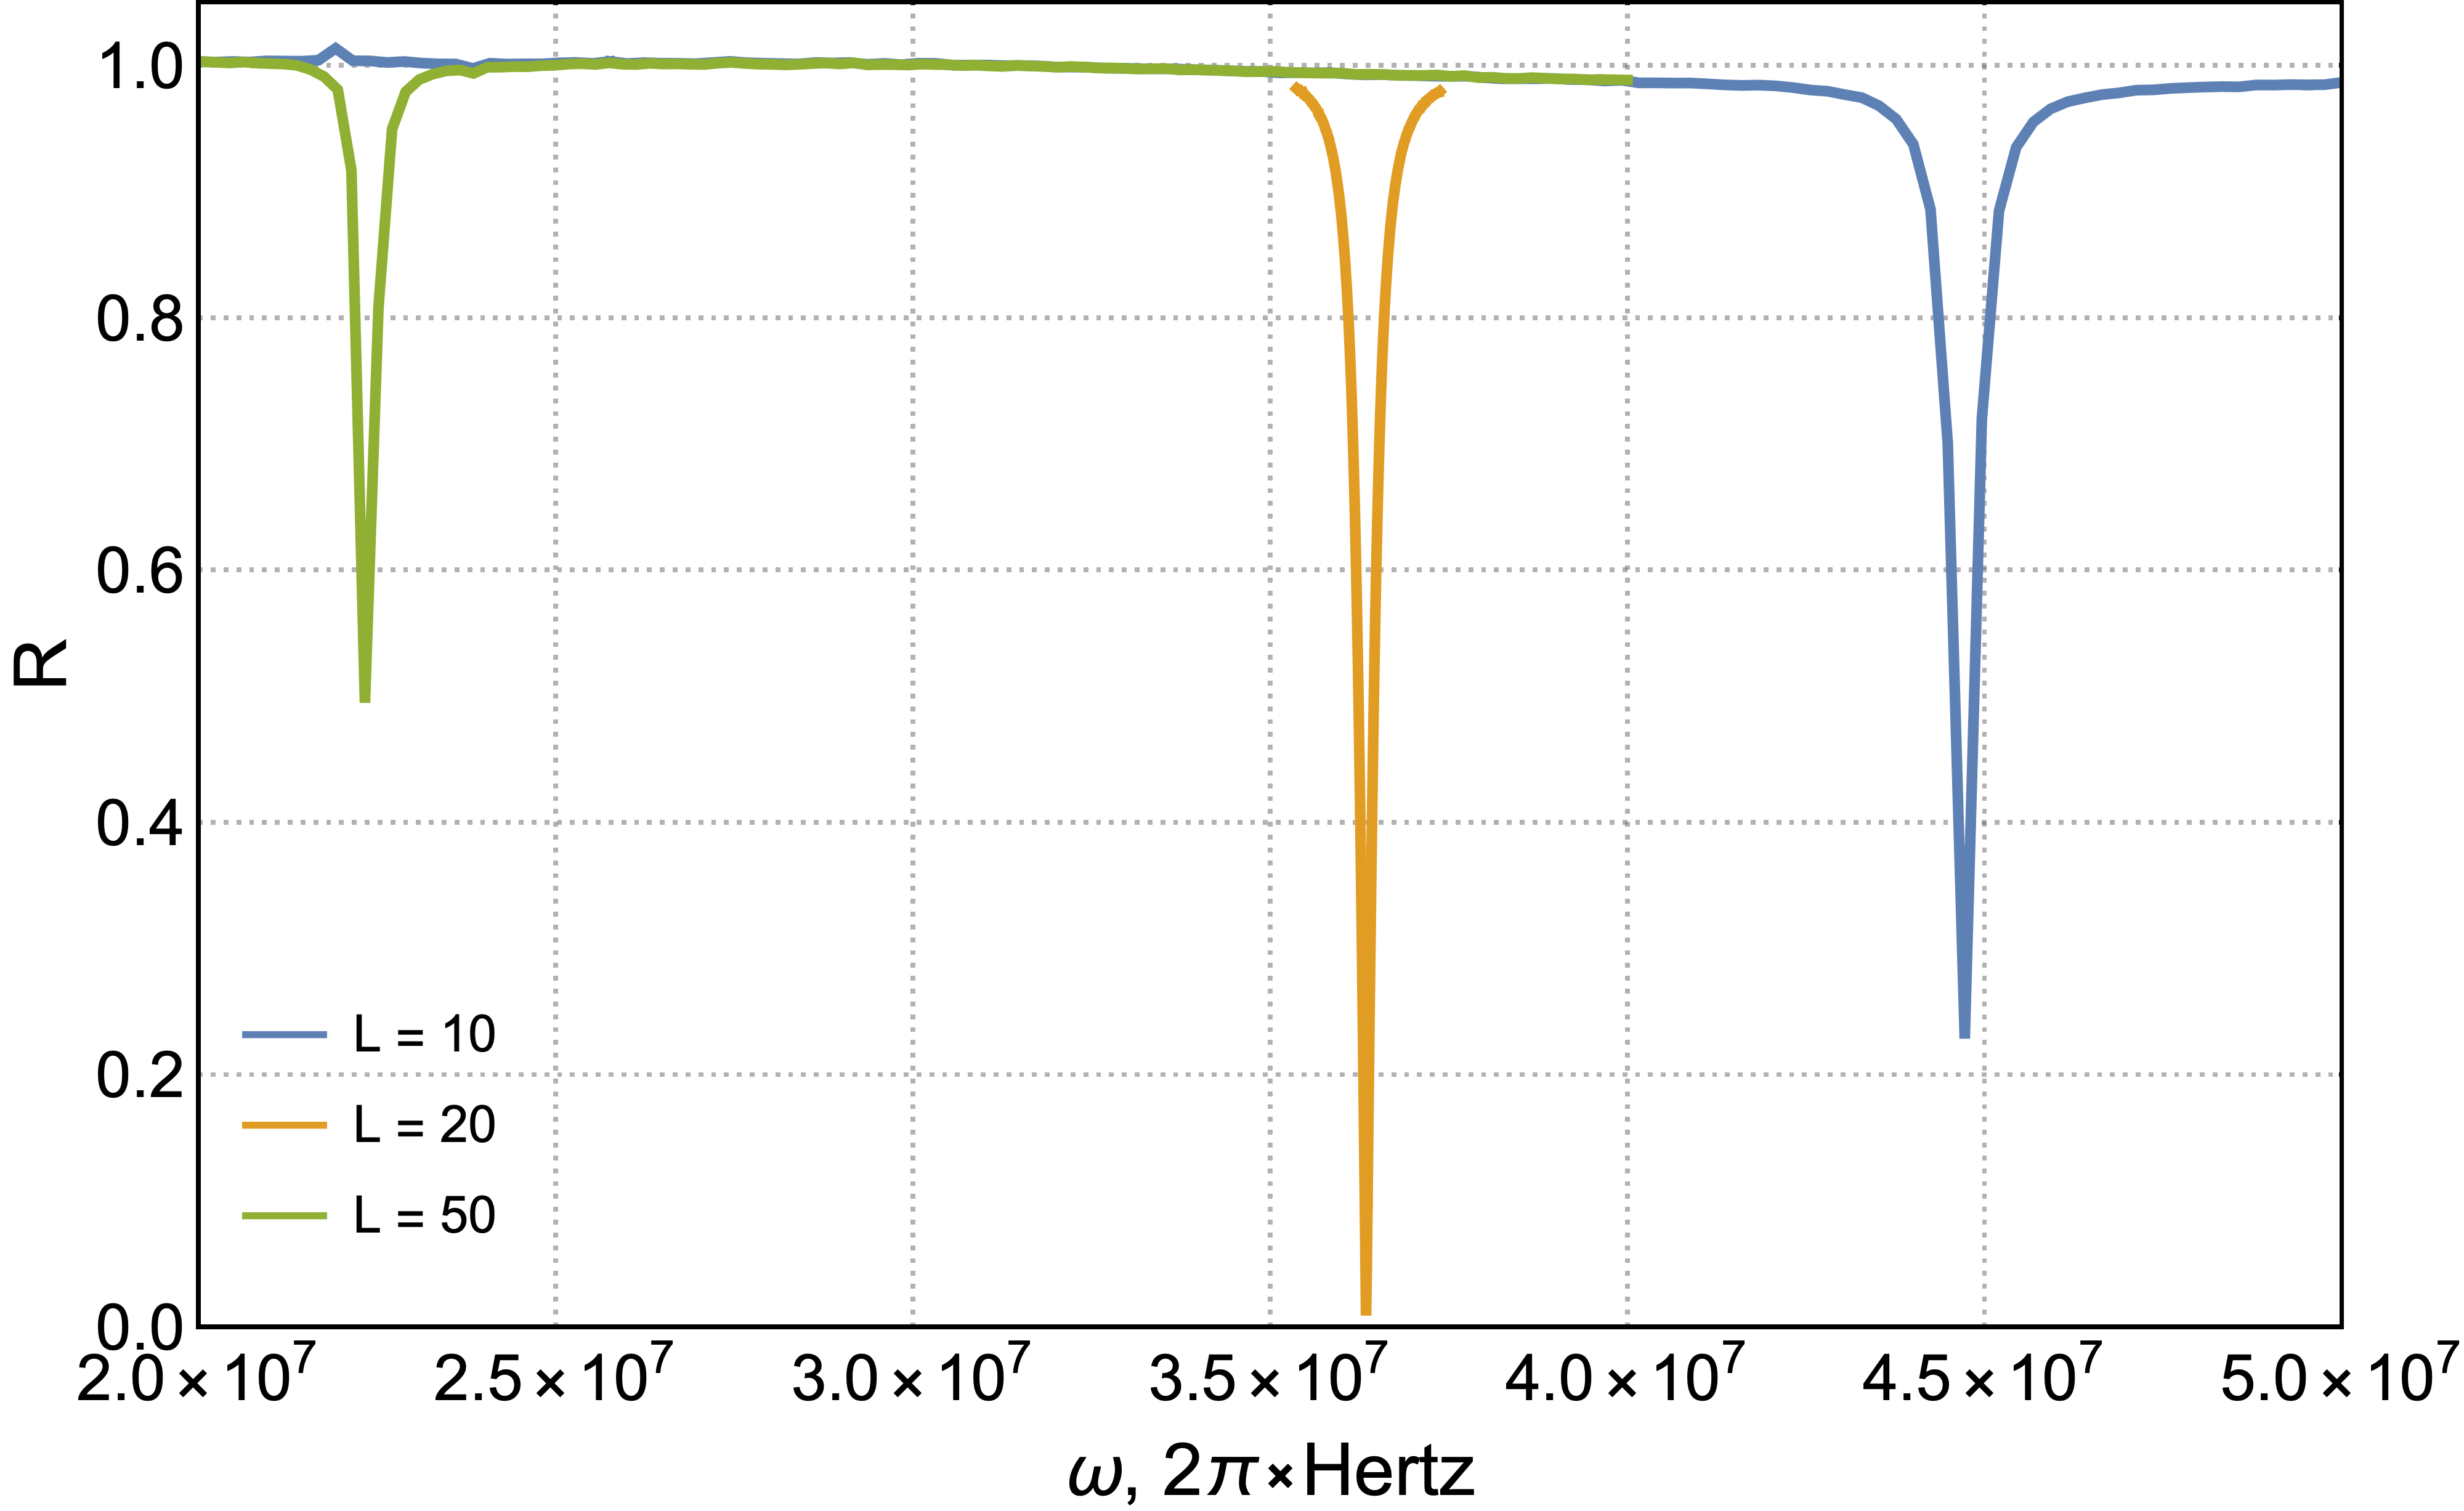
\includegraphics[width=\textwidth]{images/R_plot_C_10}
	\label{fig:R_C_10}
	\caption{Reflection spectrum for $C = 10$}
\end{figure}
\begin{figure}[h]
	\centering
	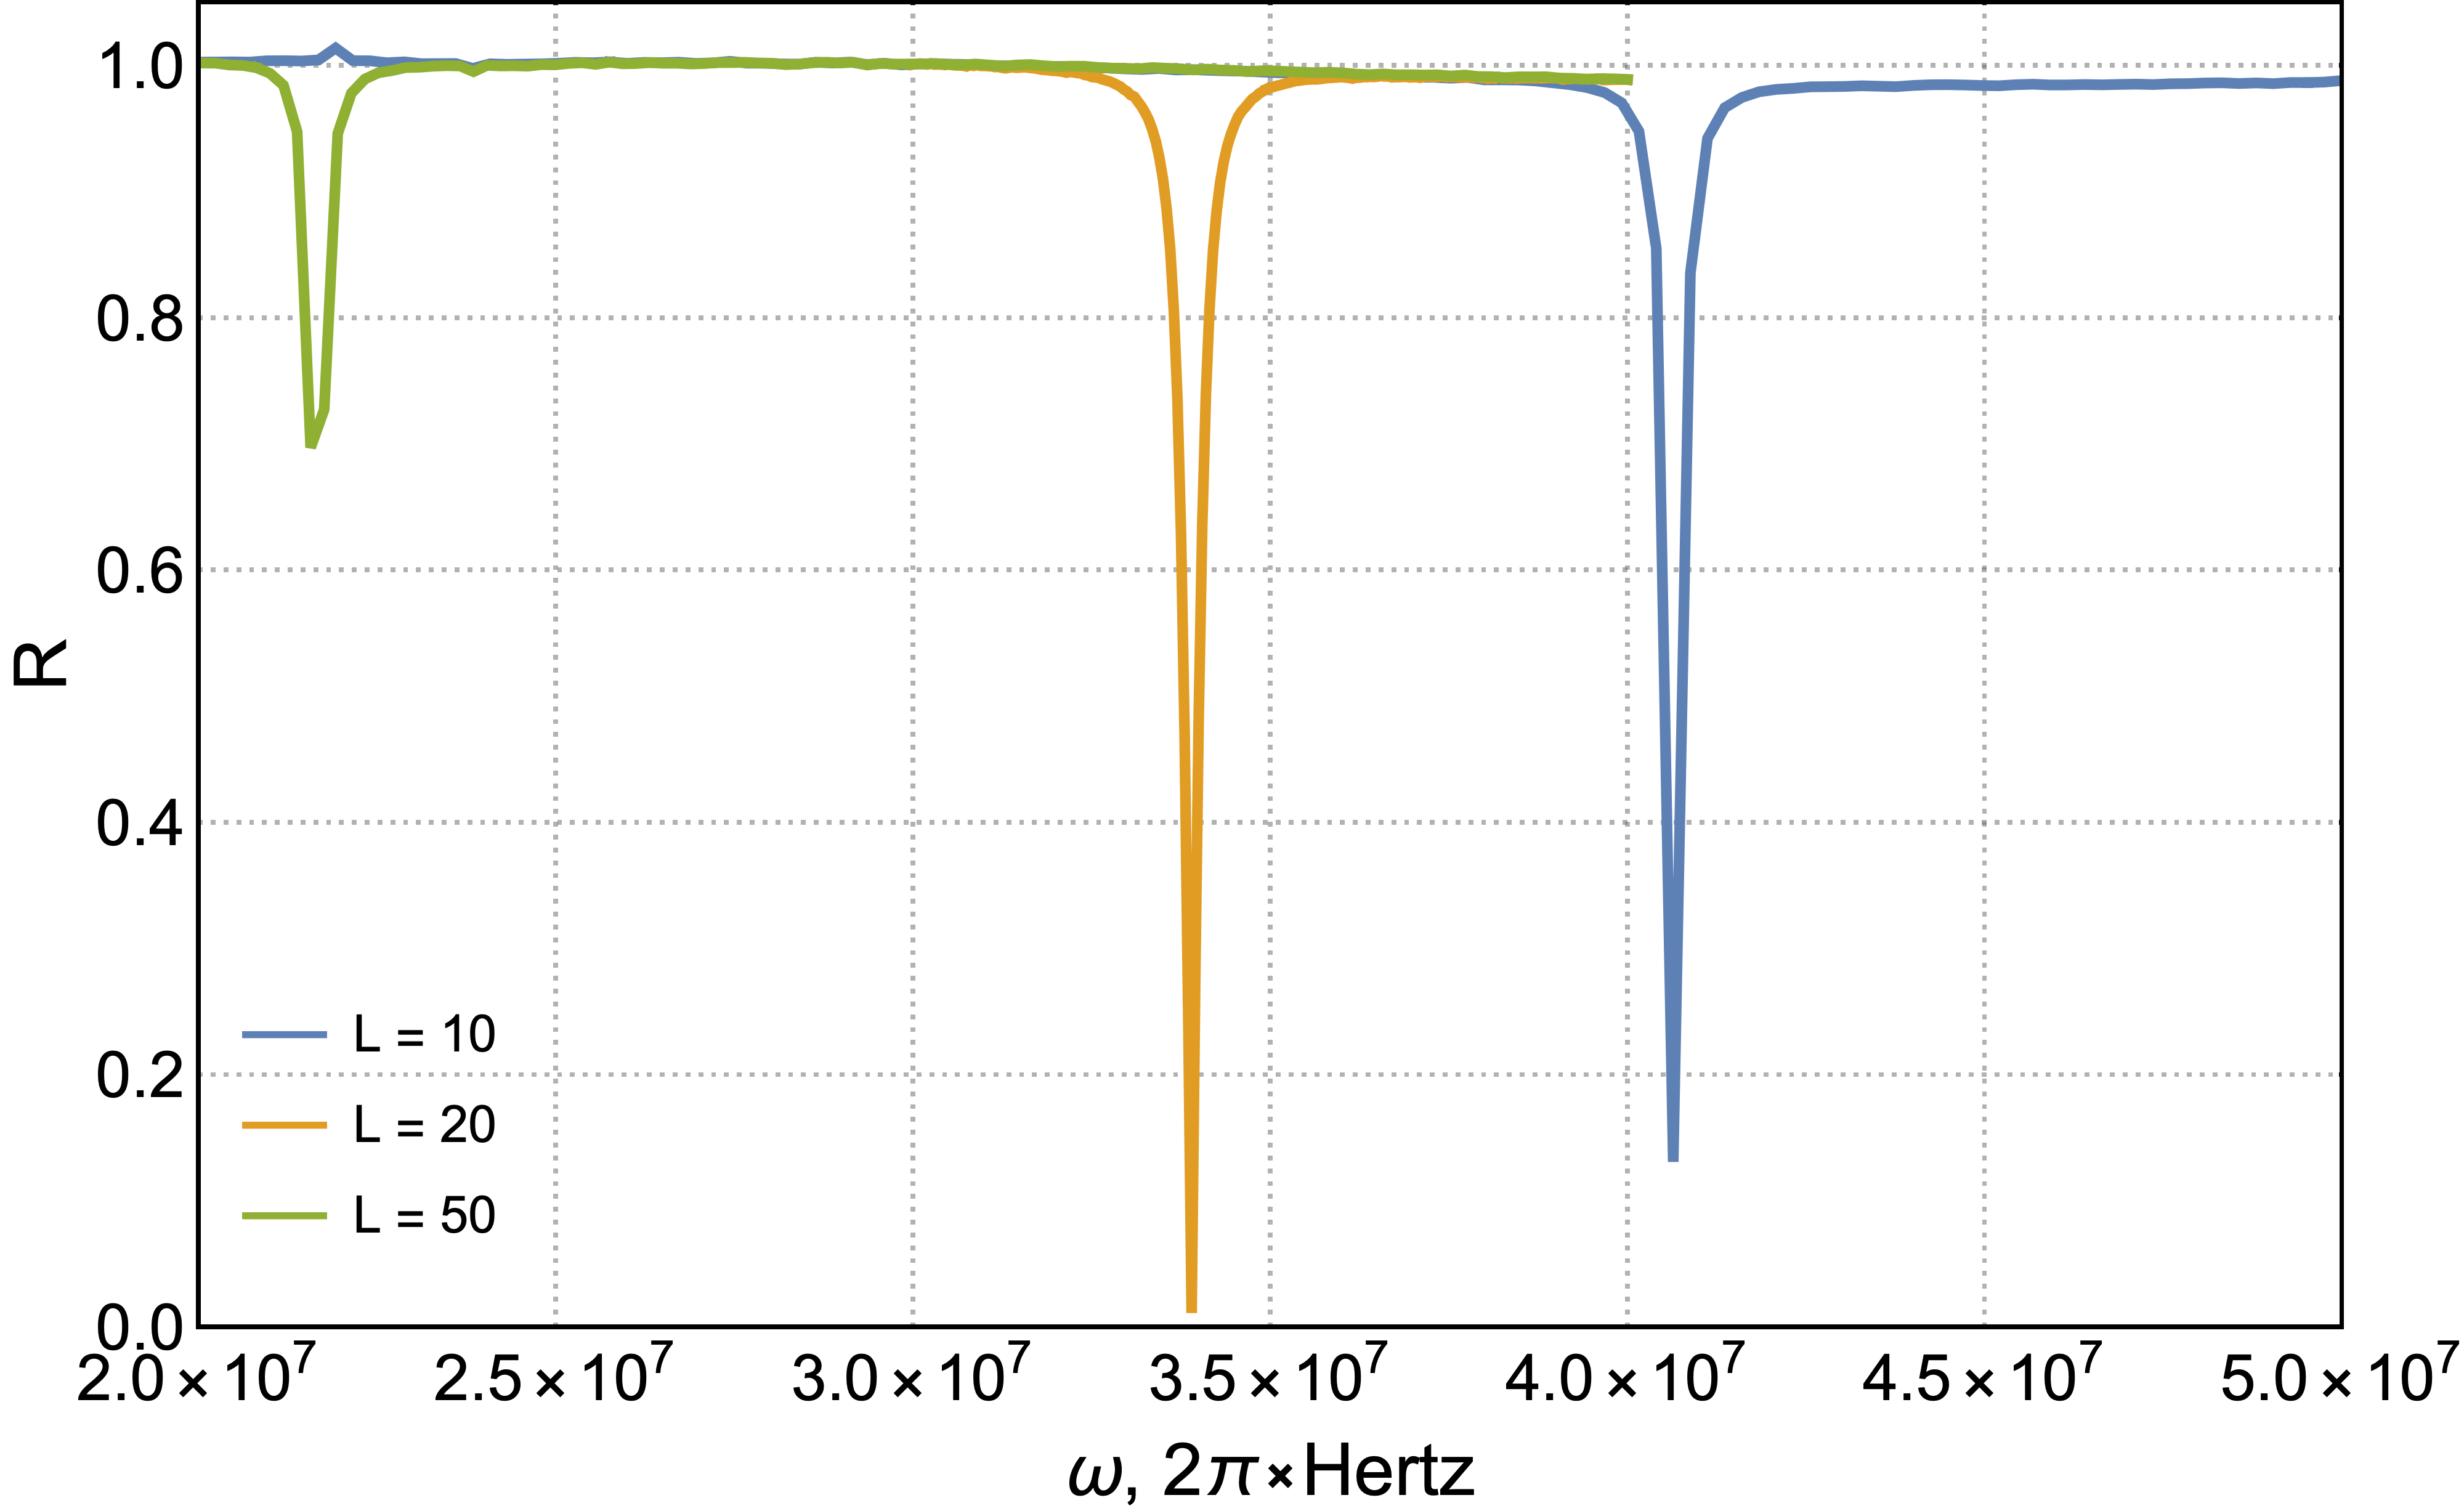
\includegraphics[width=\textwidth]{images/R_plot_C_15}
	\label{fig:R_C_10}
	\caption{Reflection spectrum for $C = 15$}
\end{figure}
\FloatBarrier
\begin{figure}[h]
	\centering
	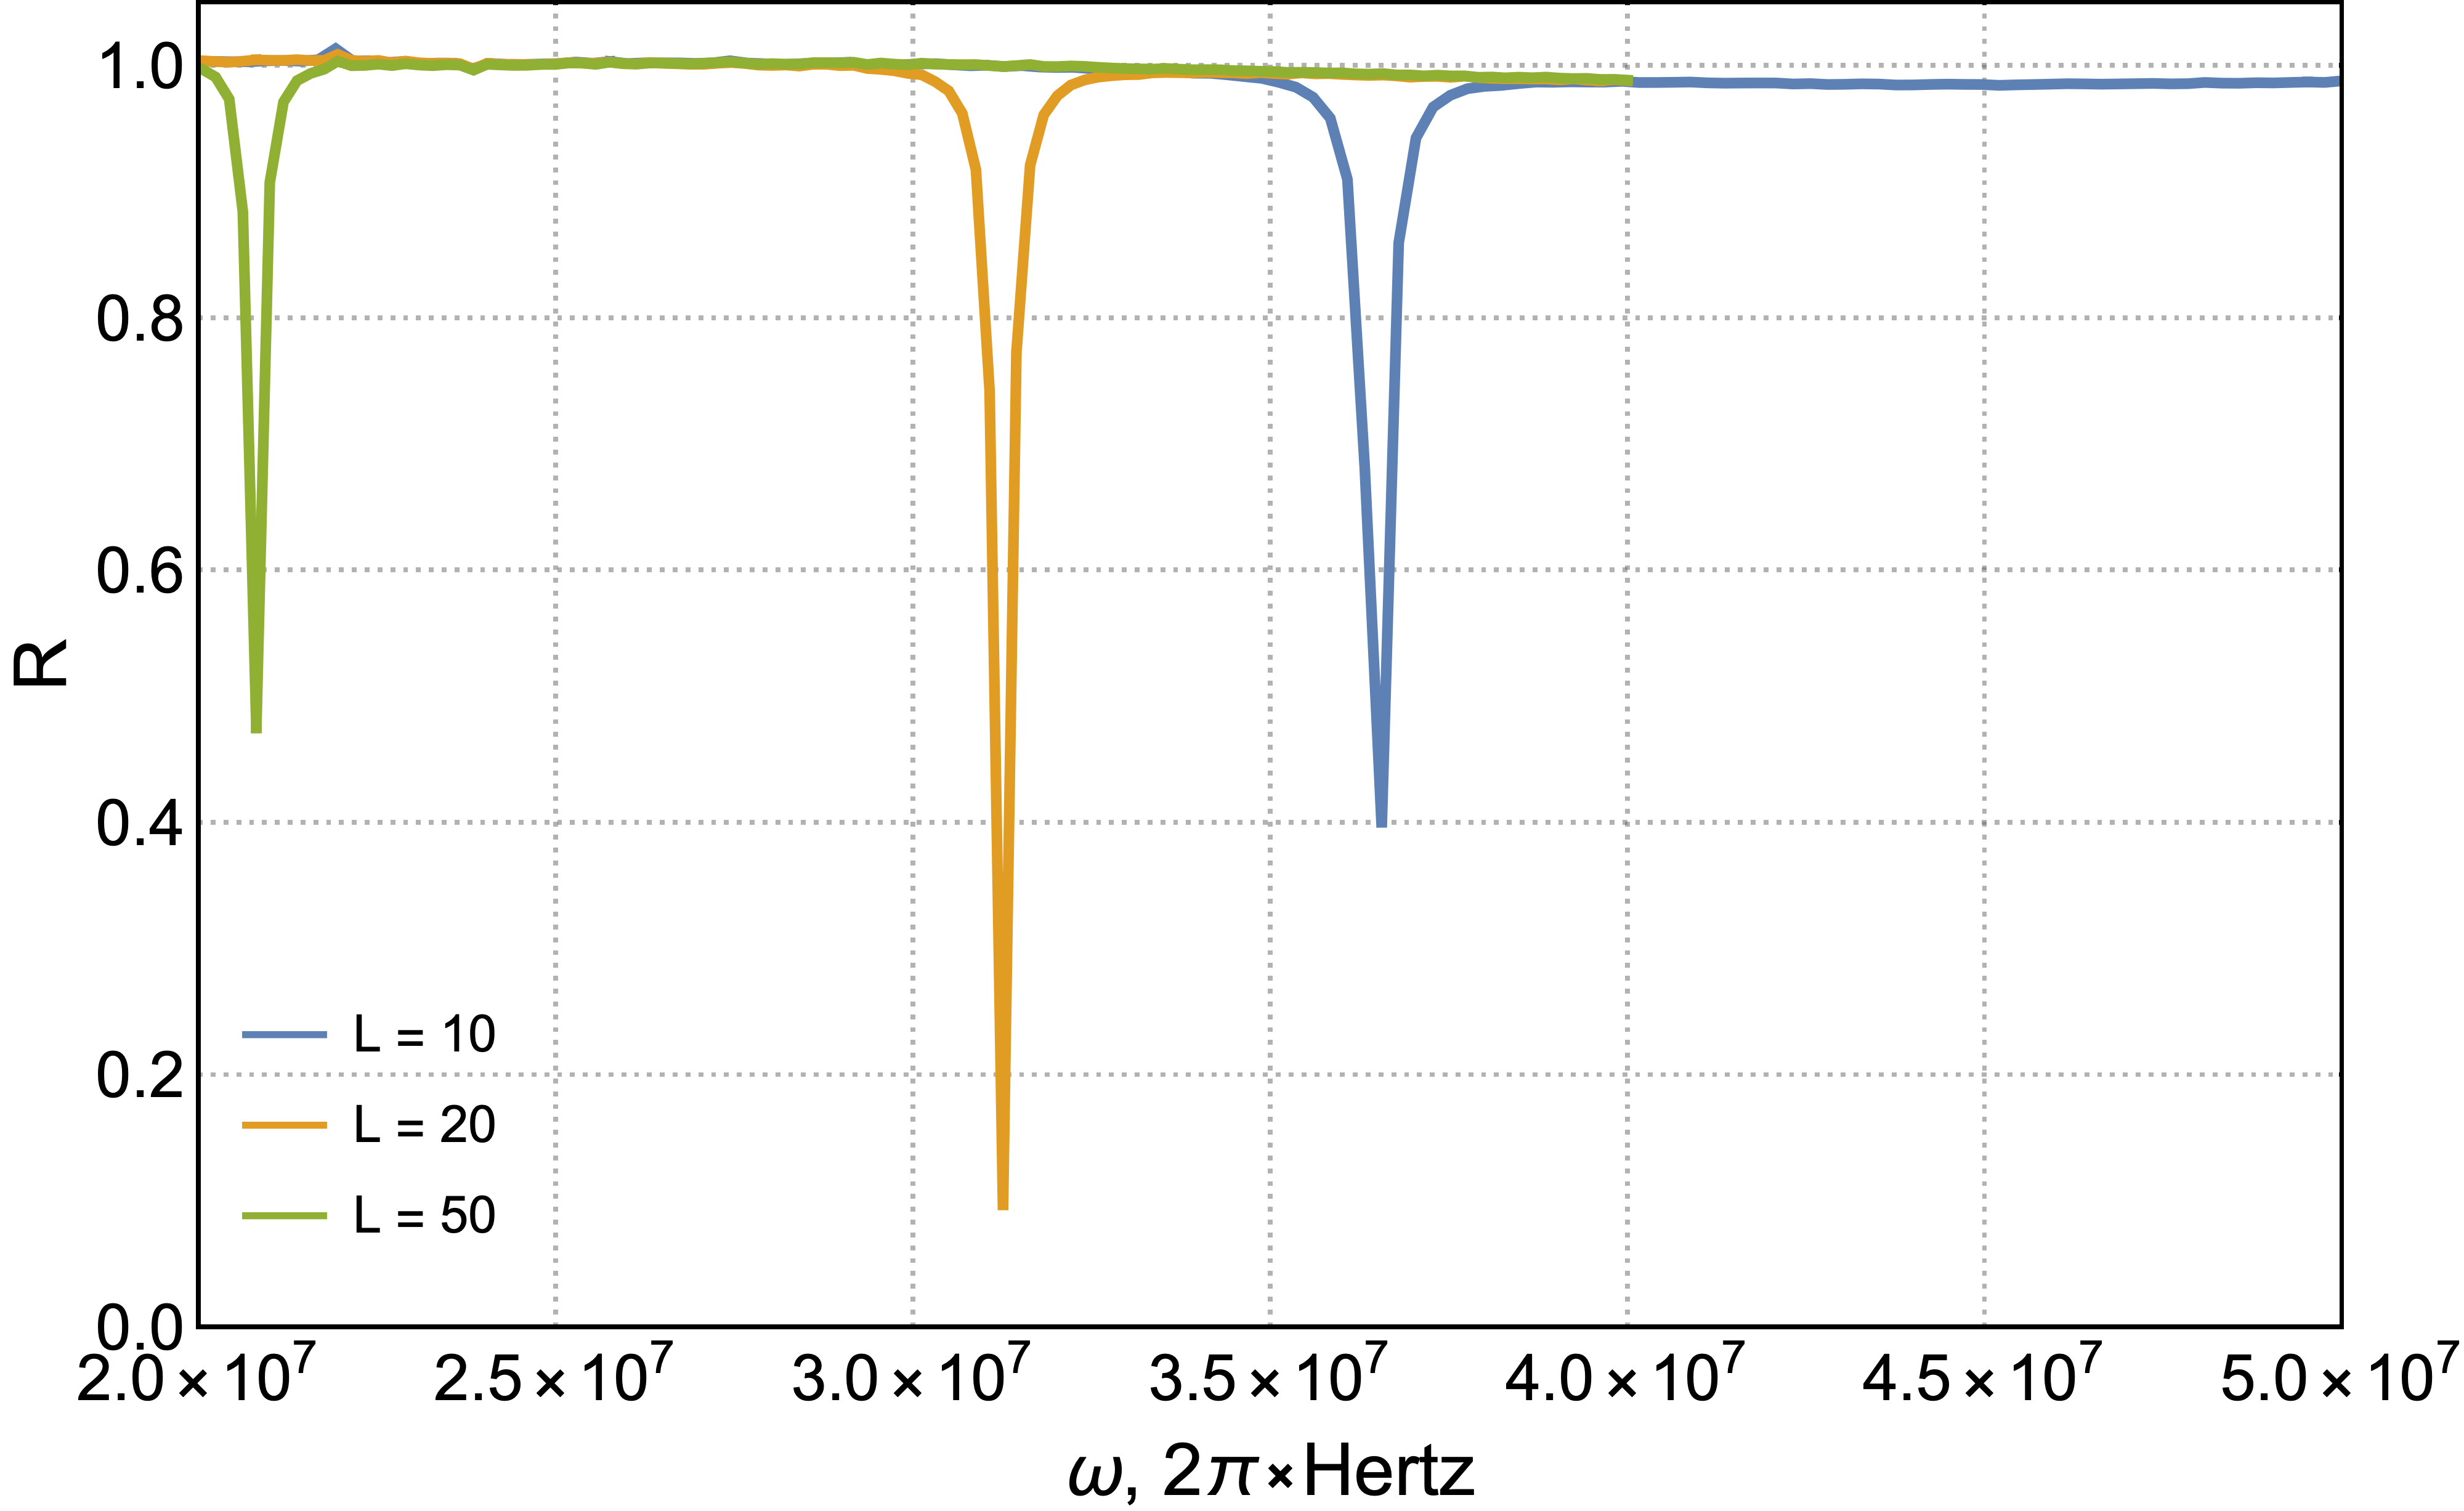
\includegraphics[width=\textwidth]{images/R_plot_C_22}
	\label{fig:R_C_10}
	\caption{Reflection spectrum for $C = 22$}
\end{figure}
\origsection{Analysis}
\FloatBarrier
Finding $\omega_0$ from experimental data is trivial, it is the central frequency of the peak. For the transmission spectrum $Q$ can be defined as
\begin{equation}
	Q = \frac{\omega_0}{\Delta \omega},
\end{equation}
where $\Delta \omega$ is the width of the peak at the $1/\sqrt{2}$ height. Since we are working with the reflection spectrum we need to adjust the height using the following expression
\begin{equation}
	R_{1/\sqrt{2}} = 1 - \frac{1 - R_{peak}}{\sqrt{2}}.
	\label{eq:reflection_height}
\end{equation}

Measured values of $\omega_0$ and $Q$ are presented in the table \ref{tbl:Q_w_results}. Visual comparison with the predicted values from the table \ref{tbl:restrictions_siverns} is shown in the chart \ref{fig:Q_w_deviation}. $C_{load} = 22$ pF is not equal to the simulated $C_{trap} = 20$ pF but was considered being close enough. The closer experimental data is to the point $\{0; 0\}$ the better it reflects the simulations. It can be seen that increased capacitance due to both $C_{load}$ and $L_{coax}$ tends to increase deviations from predictions. Our model does not account for the additional capacitances and resistances of the SMA connectors and the wires. Thus the predicted values in the table \ref{tbl:Q_w_results} are expected to be independent of the wire length and the number of SMA connectors with ``\dittotikz'' standing for the ``same as above''.
\begin{table}[h]
\centering
\begin{tabular}{| r | r || r | r || r | r |}
	\hline
	$C_{load}$, pF & $L_{coax}$, cm & $\omega^{simul}_0$, $2\pi*$MHz & $\omega_0$, $2\pi*$MHz & $Q^{simul}$ & $Q$\\
	\hline \hline
	10 & 10 & 44.6 & 44.7 & 418 & 223.5\\
	\hline
	10 & 20 & \dittotikz & 36.3 & \dittotikz & 269.9\\
	\hline
	10 & 50 & \dittotikz & 22.3 & \dittotikz & 140.4\\
	\hline
	15 & 10 & 45.6 & 40.6 & 360 & 216.5\\
	\hline
	15 & 20 & \dittotikz & 33.9 & \dittotikz & 268.6\\
	\hline
	15 & 50 & \dittotikz & 21.6 & \dittotikz & 69.7\\
	\hline
	22 & 10 & 46.9 & 36.5 & 311 & 153.5\\
	\hline
	22 & 20 & \dittotikz & 31.2 & \dittotikz & 192.3\\
	\hline
	22 & 50 & \dittotikz & 20.8 & \dittotikz & 145.6\\
	\hline
\end{tabular}
\label{tbl:Q_w_results}
\caption{Measured $Q$ and $\omega_0$ for various configurations}
\end{table}

\begin{figure}[h]
	\centering
	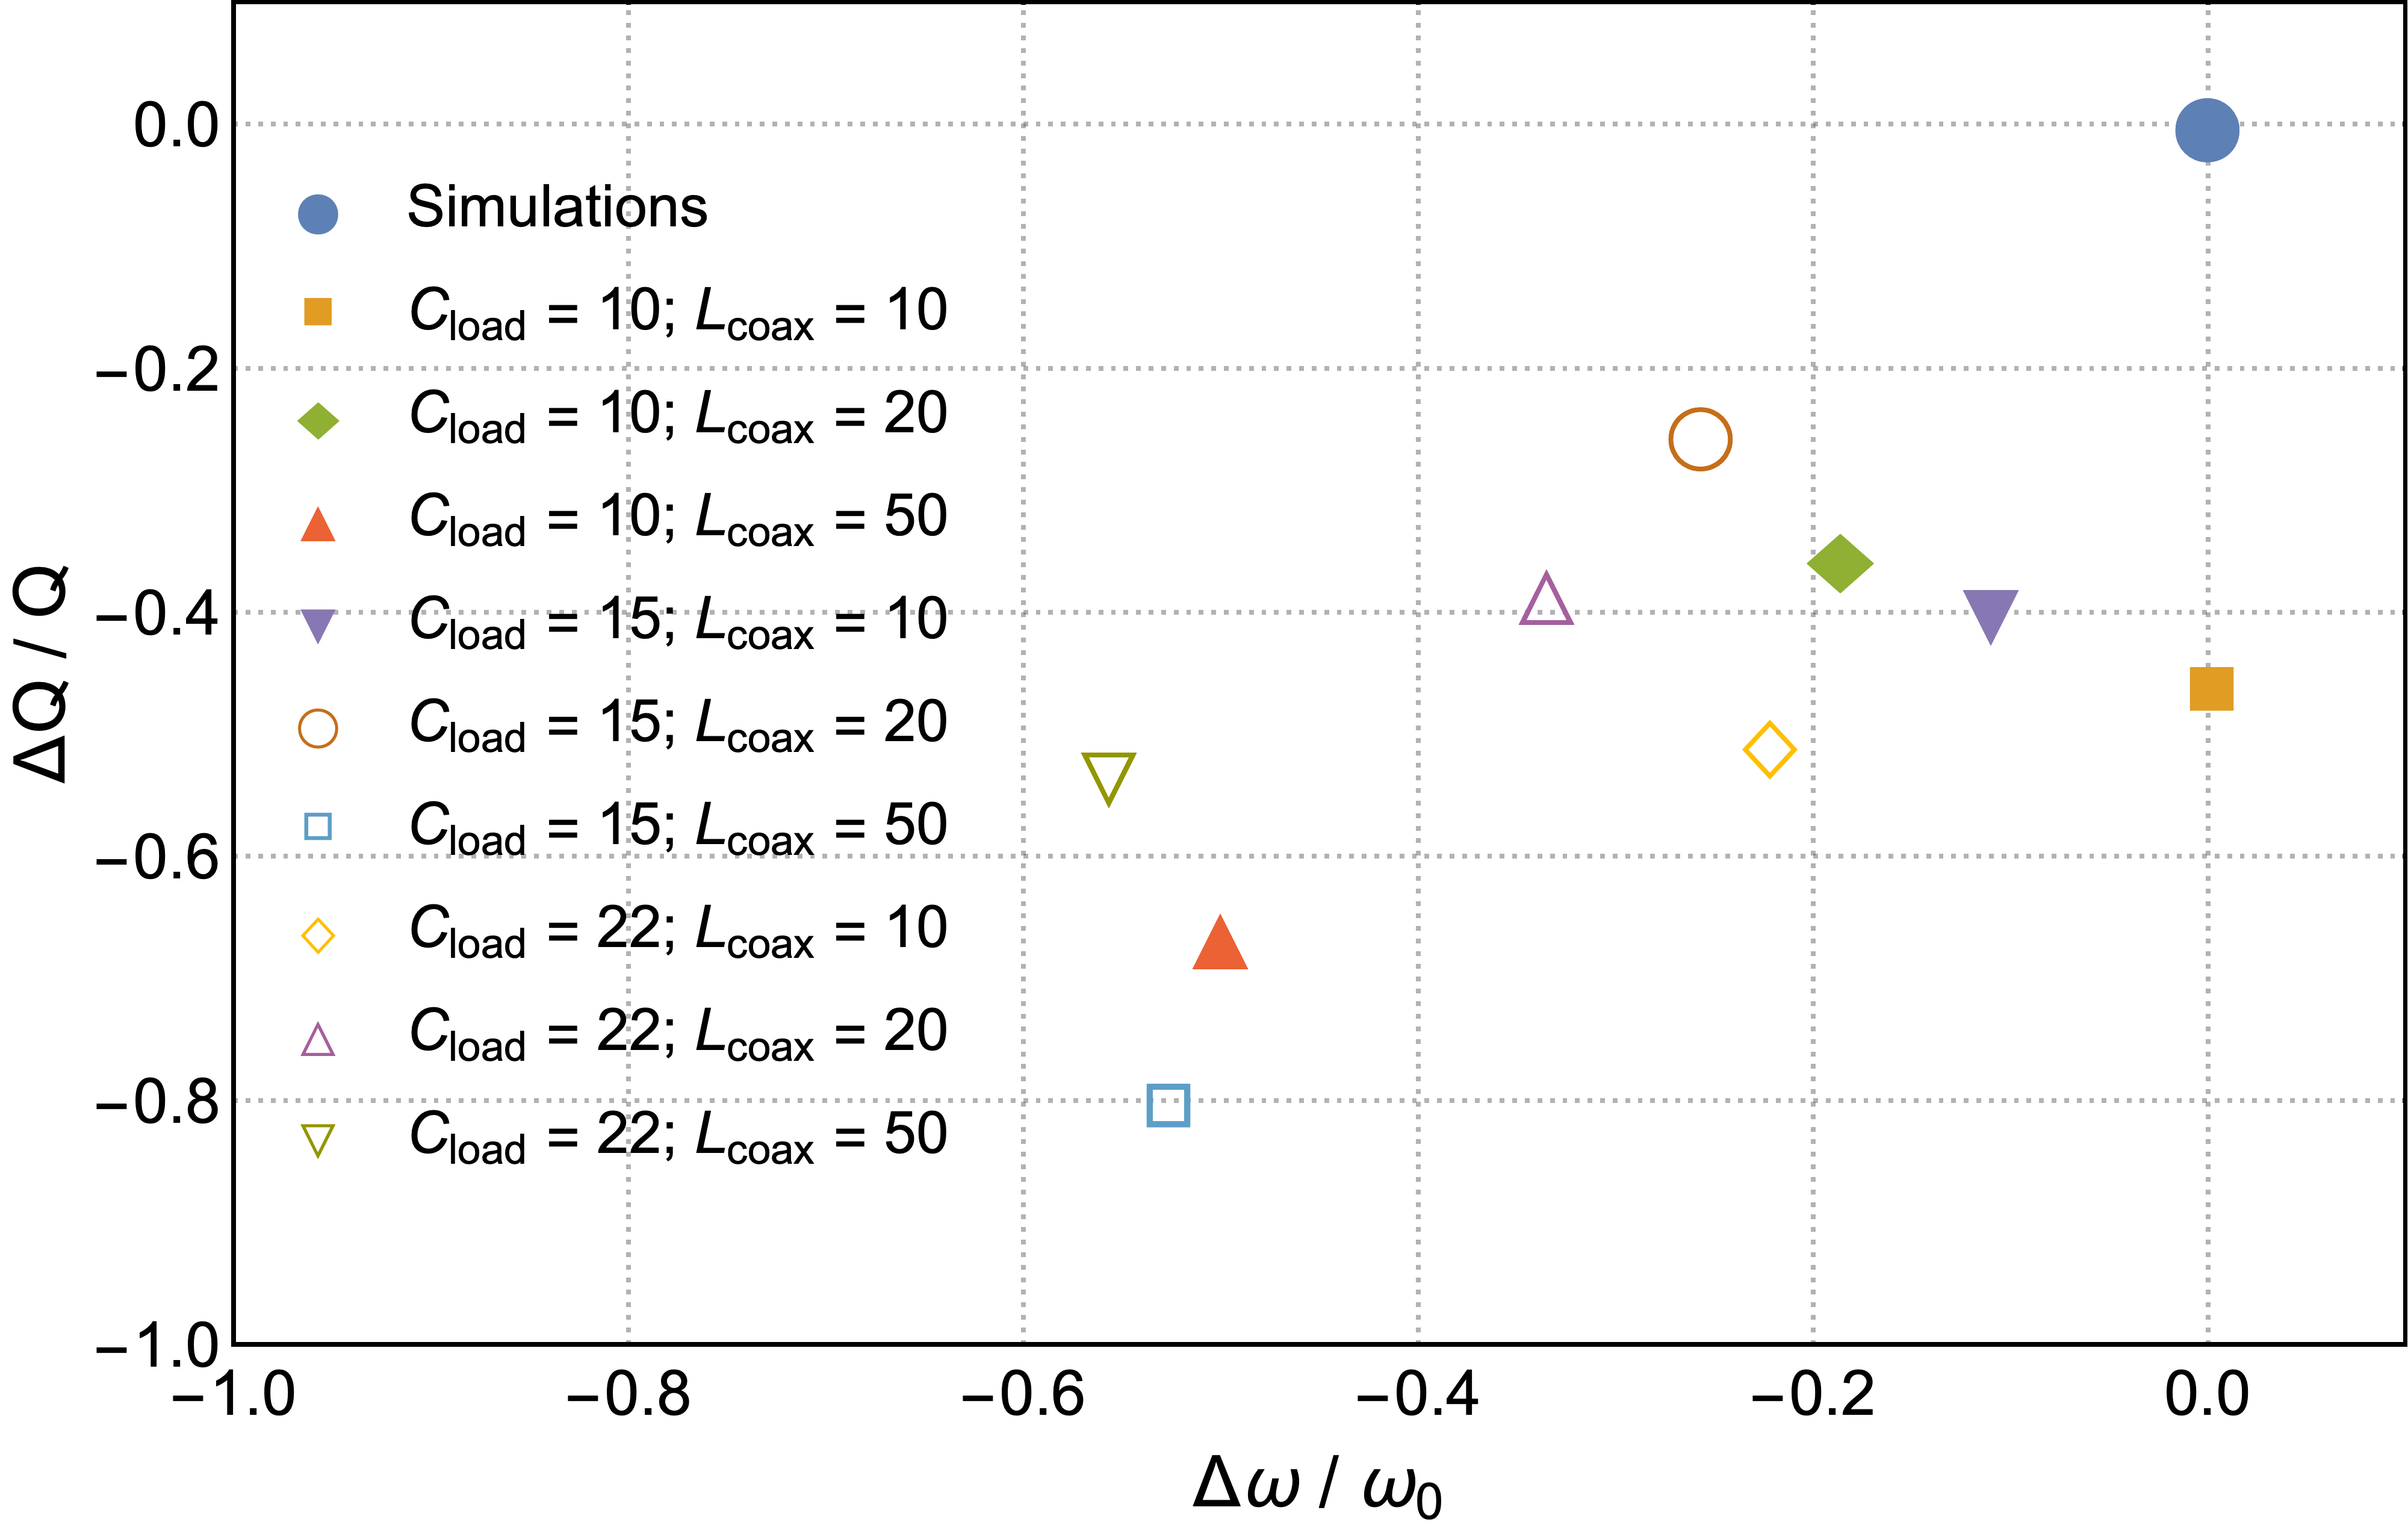
\includegraphics[width=\textwidth]{images/Q_w_plot}
	\label{fig:Q_w_deviation}
	\caption{Relative deviations of $Q$ and $\omega_0$}
\end{figure}

\section{Ideal drive}
This section includes simulations of the ideal drive for a 300 and 320 V drive by Chiara Decaroli, figures \ref{fig:ideal_drive_300} and \ref{fig:ideal_drive_320} respectively. Let's take a look at the figure \ref{fig:ideal_drive_300}. If the resonator frequency is below $\approx 2\pi*34$ MHz the ion trap becomes unstable. On the other hand, with frequencies larger than $\approx 2\pi*39$ MHz the secular frequency of the ion itself drops below $2\pi*6$ MHz which does not allow certain quantum operations. Thus it is desired for the $\omega_0$ to belong to the intersection of the white areas. We show what measured points respect this condition in the table \ref{tbl:ideal_drive}.

\begin{figure}[h]
	\centering
	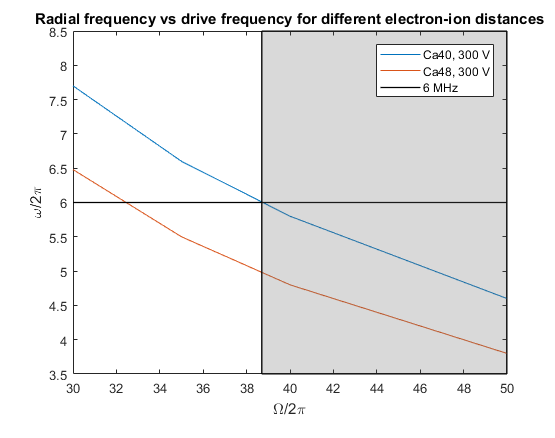
\includegraphics[width=\textwidth]{images/300V_left}
	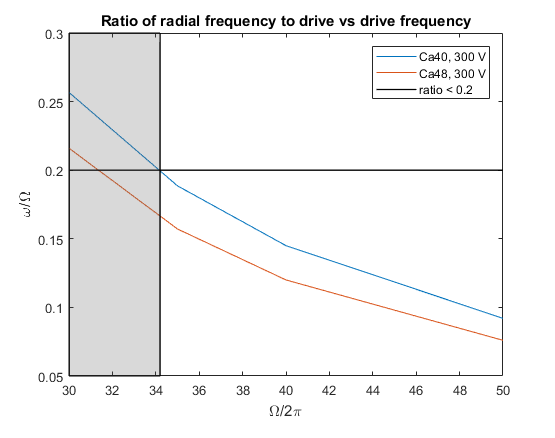
\includegraphics[width=\textwidth]{images/300V_right}
	\label{fig:ideal_drive_300}
	\caption{Simulation of the ideal drive for 300V}
\end{figure}
\begin{figure}[h]
	\centering
	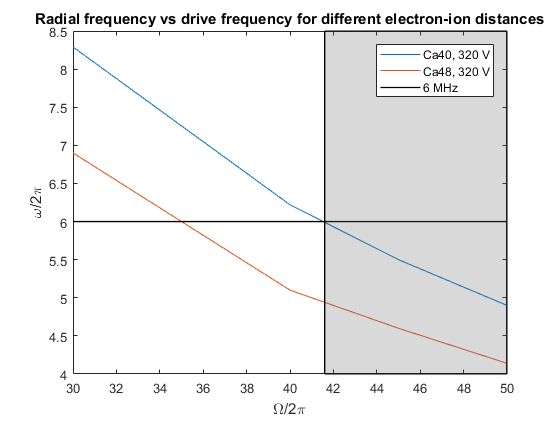
\includegraphics[width=\textwidth]{images/320V_left}
	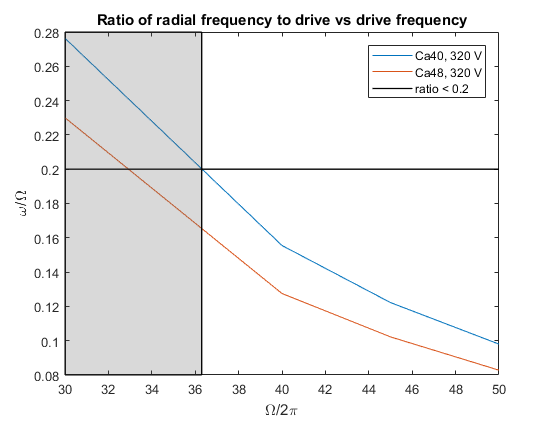
\includegraphics[width=\textwidth]{images/320V_right}
	\label{fig:ideal_drive_320}
	\caption{Simulation of the ideal drive for 320V}
\end{figure}
\FloatBarrier
\begin{table}[h]
\centering
\begin{tabular}{| r | r | c | c |}
	\hline
	$C_{load}$, pF & $L_{coax}$, cm & Compatible with 300V & Compatible with 320V\\
	\hline \hline
	10 & 10 & \xmark & \xmark\\
	\hline
	10 & 20 & \cmark & \cmark\\
	\hline
	10 & 50 & \xmark & \xmark\\
	\hline
	15 & 10 & \xmark & \cmark\\
	\hline
	15 & 20 & \cmark & \xmark\\
	\hline
	15 & 50 & \xmark & \xmark\\
	\hline
	22 & 10 & \cmark & \cmark\\
	\hline
	22 & 20 & \xmark & \xmark\\
	\hline
	22 & 50 & \xmark & \xmark\\
	\hline
\end{tabular}
\label{tbl:ideal_drive}
\caption{Fitting the experimental data into the ion trap constrains}
\end{table}

\section{Voltage gains}
According to \cite{Leupold2015} average dissipated power $P$ can be written as
\begin{equation}
	P = \frac{I_0^2 \, R}{2} = \frac{\left(U_0 \, \omega_0 \, C\right)^2 R}{2} = \frac{U_0^2}{2 \, \omega_0 \, Q  \, L}
\end{equation}
with a peak current $I_0$, peak voltage $U_0$, inductance of the resonator $L$, and capacitance of the system $C$. Since in the section \ref{sec:measurements} we made measurements with various known values of a capacitive load it is possible to give an estimation of $L = 600$ nH. By picking the values from the table \ref{tbl:ideal_drive} that are compatible with $U_0 = $ 300 or 320V we present results for the needed input power in the table \ref{tbl:input_power}.

\begin{table}[h]
\centering
\begin{tabular}{| r | r | r | r |}
	\hline
	$C_{load}$, pF & $L_{coax}$, cm & $U_0$, V & $P$, W\\
	\hline \hline
	10 & 20 & 300 & 1.20\\
	\hline
	10 & 20 & 320 & 1.37\\
	\hline
	15 & 10 & 320 & 1.53\\
	\hline
	15 & 20 & 300 & 1.30\\
	\hline
	22 & 10 & 300 & 2.11\\
	\hline
	22 & 10 & 320 & 2.40\\
	\hline
\end{tabular}
\label{tbl:input_power}
\caption{Estimated input power $P$ for various configurations}
\end{table}